\documentclass[tikz,border=8pt]{standalone}
\usepackage[utf8]{inputenc}
\usepackage[OT4,plmath]{polski}
\usepackage{amsmath}
\begin{document}
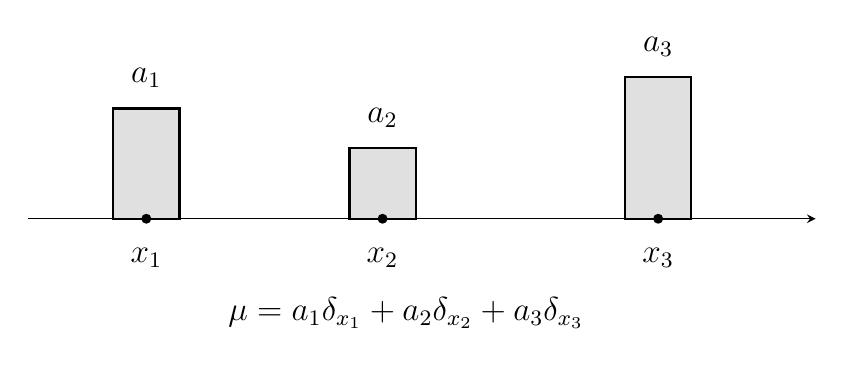
\begin{tikzpicture}[font=\large,>=stealth]
  \draw[->] (0,0)--(10,0);
  \foreach \x/\h/\i in {1.5/1.4/1,4.5/.9/2,8/1.8/3} {
    \fill[black!12] (\x-.42,0) rectangle (\x+.42,\h);
    \draw[thick] (\x-.42,0) rectangle (\x+.42,\h);
    \fill (\x,0) circle (1.8pt);
    \node[below=7pt] at (\x,0) {$x_{\i}$};
    \node[above=4pt] at (\x,\h) {$a_{\i}$};
  }
  \node at (4.8,-1.2)
    {$\mu=a_1\delta_{x_1}+a_2\delta_{x_2}+a_3\delta_{x_3}$};
\end{tikzpicture}
\end{document}
